
% Default to the notebook output style

    


% Inherit from the specified cell style.




    
\documentclass[11pt]{article}

    
    
    \usepackage[T1]{fontenc}
    % Nicer default font (+ math font) than Computer Modern for most use cases
    \usepackage{mathpazo}

    % Basic figure setup, for now with no caption control since it's done
    % automatically by Pandoc (which extracts ![](path) syntax from Markdown).
    \usepackage{graphicx}
    % We will generate all images so they have a width \maxwidth. This means
    % that they will get their normal width if they fit onto the page, but
    % are scaled down if they would overflow the margins.
    \makeatletter
    \def\maxwidth{\ifdim\Gin@nat@width>\linewidth\linewidth
    \else\Gin@nat@width\fi}
    \makeatother
    \let\Oldincludegraphics\includegraphics
    % Set max figure width to be 80% of text width, for now hardcoded.
    \renewcommand{\includegraphics}[1]{\Oldincludegraphics[width=.8\maxwidth]{#1}}
    % Ensure that by default, figures have no caption (until we provide a
    % proper Figure object with a Caption API and a way to capture that
    % in the conversion process - todo).
    \usepackage{caption}
    \DeclareCaptionLabelFormat{nolabel}{}
    \captionsetup{labelformat=nolabel}

    \usepackage{adjustbox} % Used to constrain images to a maximum size 
    \usepackage{xcolor} % Allow colors to be defined
    \usepackage{enumerate} % Needed for markdown enumerations to work
    \usepackage{geometry} % Used to adjust the document margins
    \usepackage{amsmath} % Equations
    \usepackage{amssymb} % Equations
    \usepackage{textcomp} % defines textquotesingle
    % Hack from http://tex.stackexchange.com/a/47451/13684:
    \AtBeginDocument{%
        \def\PYZsq{\textquotesingle}% Upright quotes in Pygmentized code
    }
    \usepackage{upquote} % Upright quotes for verbatim code
    \usepackage{eurosym} % defines \euro
    \usepackage[mathletters]{ucs} % Extended unicode (utf-8) support
    \usepackage[utf8x]{inputenc} % Allow utf-8 characters in the tex document
    \usepackage{fancyvrb} % verbatim replacement that allows latex
    \usepackage{grffile} % extends the file name processing of package graphics 
                         % to support a larger range 
    % The hyperref package gives us a pdf with properly built
    % internal navigation ('pdf bookmarks' for the table of contents,
    % internal cross-reference links, web links for URLs, etc.)
    \usepackage{hyperref}
    \usepackage{longtable} % longtable support required by pandoc >1.10
    \usepackage{booktabs}  % table support for pandoc > 1.12.2
    \usepackage[inline]{enumitem} % IRkernel/repr support (it uses the enumerate* environment)
    \usepackage[normalem]{ulem} % ulem is needed to support strikethroughs (\sout)
                                % normalem makes italics be italics, not underlines
    

    
    
    % Colors for the hyperref package
    \definecolor{urlcolor}{rgb}{0,.145,.698}
    \definecolor{linkcolor}{rgb}{.71,0.21,0.01}
    \definecolor{citecolor}{rgb}{.12,.54,.11}

    % ANSI colors
    \definecolor{ansi-black}{HTML}{3E424D}
    \definecolor{ansi-black-intense}{HTML}{282C36}
    \definecolor{ansi-red}{HTML}{E75C58}
    \definecolor{ansi-red-intense}{HTML}{B22B31}
    \definecolor{ansi-green}{HTML}{00A250}
    \definecolor{ansi-green-intense}{HTML}{007427}
    \definecolor{ansi-yellow}{HTML}{DDB62B}
    \definecolor{ansi-yellow-intense}{HTML}{B27D12}
    \definecolor{ansi-blue}{HTML}{208FFB}
    \definecolor{ansi-blue-intense}{HTML}{0065CA}
    \definecolor{ansi-magenta}{HTML}{D160C4}
    \definecolor{ansi-magenta-intense}{HTML}{A03196}
    \definecolor{ansi-cyan}{HTML}{60C6C8}
    \definecolor{ansi-cyan-intense}{HTML}{258F8F}
    \definecolor{ansi-white}{HTML}{C5C1B4}
    \definecolor{ansi-white-intense}{HTML}{A1A6B2}

    % commands and environments needed by pandoc snippets
    % extracted from the output of `pandoc -s`
    \providecommand{\tightlist}{%
      \setlength{\itemsep}{0pt}\setlength{\parskip}{0pt}}
    \DefineVerbatimEnvironment{Highlighting}{Verbatim}{commandchars=\\\{\}}
    % Add ',fontsize=\small' for more characters per line
    \newenvironment{Shaded}{}{}
    \newcommand{\KeywordTok}[1]{\textcolor[rgb]{0.00,0.44,0.13}{\textbf{{#1}}}}
    \newcommand{\DataTypeTok}[1]{\textcolor[rgb]{0.56,0.13,0.00}{{#1}}}
    \newcommand{\DecValTok}[1]{\textcolor[rgb]{0.25,0.63,0.44}{{#1}}}
    \newcommand{\BaseNTok}[1]{\textcolor[rgb]{0.25,0.63,0.44}{{#1}}}
    \newcommand{\FloatTok}[1]{\textcolor[rgb]{0.25,0.63,0.44}{{#1}}}
    \newcommand{\CharTok}[1]{\textcolor[rgb]{0.25,0.44,0.63}{{#1}}}
    \newcommand{\StringTok}[1]{\textcolor[rgb]{0.25,0.44,0.63}{{#1}}}
    \newcommand{\CommentTok}[1]{\textcolor[rgb]{0.38,0.63,0.69}{\textit{{#1}}}}
    \newcommand{\OtherTok}[1]{\textcolor[rgb]{0.00,0.44,0.13}{{#1}}}
    \newcommand{\AlertTok}[1]{\textcolor[rgb]{1.00,0.00,0.00}{\textbf{{#1}}}}
    \newcommand{\FunctionTok}[1]{\textcolor[rgb]{0.02,0.16,0.49}{{#1}}}
    \newcommand{\RegionMarkerTok}[1]{{#1}}
    \newcommand{\ErrorTok}[1]{\textcolor[rgb]{1.00,0.00,0.00}{\textbf{{#1}}}}
    \newcommand{\NormalTok}[1]{{#1}}
    
    % Additional commands for more recent versions of Pandoc
    \newcommand{\ConstantTok}[1]{\textcolor[rgb]{0.53,0.00,0.00}{{#1}}}
    \newcommand{\SpecialCharTok}[1]{\textcolor[rgb]{0.25,0.44,0.63}{{#1}}}
    \newcommand{\VerbatimStringTok}[1]{\textcolor[rgb]{0.25,0.44,0.63}{{#1}}}
    \newcommand{\SpecialStringTok}[1]{\textcolor[rgb]{0.73,0.40,0.53}{{#1}}}
    \newcommand{\ImportTok}[1]{{#1}}
    \newcommand{\DocumentationTok}[1]{\textcolor[rgb]{0.73,0.13,0.13}{\textit{{#1}}}}
    \newcommand{\AnnotationTok}[1]{\textcolor[rgb]{0.38,0.63,0.69}{\textbf{\textit{{#1}}}}}
    \newcommand{\CommentVarTok}[1]{\textcolor[rgb]{0.38,0.63,0.69}{\textbf{\textit{{#1}}}}}
    \newcommand{\VariableTok}[1]{\textcolor[rgb]{0.10,0.09,0.49}{{#1}}}
    \newcommand{\ControlFlowTok}[1]{\textcolor[rgb]{0.00,0.44,0.13}{\textbf{{#1}}}}
    \newcommand{\OperatorTok}[1]{\textcolor[rgb]{0.40,0.40,0.40}{{#1}}}
    \newcommand{\BuiltInTok}[1]{{#1}}
    \newcommand{\ExtensionTok}[1]{{#1}}
    \newcommand{\PreprocessorTok}[1]{\textcolor[rgb]{0.74,0.48,0.00}{{#1}}}
    \newcommand{\AttributeTok}[1]{\textcolor[rgb]{0.49,0.56,0.16}{{#1}}}
    \newcommand{\InformationTok}[1]{\textcolor[rgb]{0.38,0.63,0.69}{\textbf{\textit{{#1}}}}}
    \newcommand{\WarningTok}[1]{\textcolor[rgb]{0.38,0.63,0.69}{\textbf{\textit{{#1}}}}}
    
    
    % Define a nice break command that doesn't care if a line doesn't already
    % exist.
    \def\br{\hspace*{\fill} \\* }
    % Math Jax compatability definitions
    \def\gt{>}
    \def\lt{<}
    % Document parameters
    \title{BiotaEvolver\_tutorial}
    
    
    

    % Pygments definitions
    
\makeatletter
\def\PY@reset{\let\PY@it=\relax \let\PY@bf=\relax%
    \let\PY@ul=\relax \let\PY@tc=\relax%
    \let\PY@bc=\relax \let\PY@ff=\relax}
\def\PY@tok#1{\csname PY@tok@#1\endcsname}
\def\PY@toks#1+{\ifx\relax#1\empty\else%
    \PY@tok{#1}\expandafter\PY@toks\fi}
\def\PY@do#1{\PY@bc{\PY@tc{\PY@ul{%
    \PY@it{\PY@bf{\PY@ff{#1}}}}}}}
\def\PY#1#2{\PY@reset\PY@toks#1+\relax+\PY@do{#2}}

\expandafter\def\csname PY@tok@w\endcsname{\def\PY@tc##1{\textcolor[rgb]{0.73,0.73,0.73}{##1}}}
\expandafter\def\csname PY@tok@c\endcsname{\let\PY@it=\textit\def\PY@tc##1{\textcolor[rgb]{0.25,0.50,0.50}{##1}}}
\expandafter\def\csname PY@tok@cp\endcsname{\def\PY@tc##1{\textcolor[rgb]{0.74,0.48,0.00}{##1}}}
\expandafter\def\csname PY@tok@k\endcsname{\let\PY@bf=\textbf\def\PY@tc##1{\textcolor[rgb]{0.00,0.50,0.00}{##1}}}
\expandafter\def\csname PY@tok@kp\endcsname{\def\PY@tc##1{\textcolor[rgb]{0.00,0.50,0.00}{##1}}}
\expandafter\def\csname PY@tok@kt\endcsname{\def\PY@tc##1{\textcolor[rgb]{0.69,0.00,0.25}{##1}}}
\expandafter\def\csname PY@tok@o\endcsname{\def\PY@tc##1{\textcolor[rgb]{0.40,0.40,0.40}{##1}}}
\expandafter\def\csname PY@tok@ow\endcsname{\let\PY@bf=\textbf\def\PY@tc##1{\textcolor[rgb]{0.67,0.13,1.00}{##1}}}
\expandafter\def\csname PY@tok@nb\endcsname{\def\PY@tc##1{\textcolor[rgb]{0.00,0.50,0.00}{##1}}}
\expandafter\def\csname PY@tok@nf\endcsname{\def\PY@tc##1{\textcolor[rgb]{0.00,0.00,1.00}{##1}}}
\expandafter\def\csname PY@tok@nc\endcsname{\let\PY@bf=\textbf\def\PY@tc##1{\textcolor[rgb]{0.00,0.00,1.00}{##1}}}
\expandafter\def\csname PY@tok@nn\endcsname{\let\PY@bf=\textbf\def\PY@tc##1{\textcolor[rgb]{0.00,0.00,1.00}{##1}}}
\expandafter\def\csname PY@tok@ne\endcsname{\let\PY@bf=\textbf\def\PY@tc##1{\textcolor[rgb]{0.82,0.25,0.23}{##1}}}
\expandafter\def\csname PY@tok@nv\endcsname{\def\PY@tc##1{\textcolor[rgb]{0.10,0.09,0.49}{##1}}}
\expandafter\def\csname PY@tok@no\endcsname{\def\PY@tc##1{\textcolor[rgb]{0.53,0.00,0.00}{##1}}}
\expandafter\def\csname PY@tok@nl\endcsname{\def\PY@tc##1{\textcolor[rgb]{0.63,0.63,0.00}{##1}}}
\expandafter\def\csname PY@tok@ni\endcsname{\let\PY@bf=\textbf\def\PY@tc##1{\textcolor[rgb]{0.60,0.60,0.60}{##1}}}
\expandafter\def\csname PY@tok@na\endcsname{\def\PY@tc##1{\textcolor[rgb]{0.49,0.56,0.16}{##1}}}
\expandafter\def\csname PY@tok@nt\endcsname{\let\PY@bf=\textbf\def\PY@tc##1{\textcolor[rgb]{0.00,0.50,0.00}{##1}}}
\expandafter\def\csname PY@tok@nd\endcsname{\def\PY@tc##1{\textcolor[rgb]{0.67,0.13,1.00}{##1}}}
\expandafter\def\csname PY@tok@s\endcsname{\def\PY@tc##1{\textcolor[rgb]{0.73,0.13,0.13}{##1}}}
\expandafter\def\csname PY@tok@sd\endcsname{\let\PY@it=\textit\def\PY@tc##1{\textcolor[rgb]{0.73,0.13,0.13}{##1}}}
\expandafter\def\csname PY@tok@si\endcsname{\let\PY@bf=\textbf\def\PY@tc##1{\textcolor[rgb]{0.73,0.40,0.53}{##1}}}
\expandafter\def\csname PY@tok@se\endcsname{\let\PY@bf=\textbf\def\PY@tc##1{\textcolor[rgb]{0.73,0.40,0.13}{##1}}}
\expandafter\def\csname PY@tok@sr\endcsname{\def\PY@tc##1{\textcolor[rgb]{0.73,0.40,0.53}{##1}}}
\expandafter\def\csname PY@tok@ss\endcsname{\def\PY@tc##1{\textcolor[rgb]{0.10,0.09,0.49}{##1}}}
\expandafter\def\csname PY@tok@sx\endcsname{\def\PY@tc##1{\textcolor[rgb]{0.00,0.50,0.00}{##1}}}
\expandafter\def\csname PY@tok@m\endcsname{\def\PY@tc##1{\textcolor[rgb]{0.40,0.40,0.40}{##1}}}
\expandafter\def\csname PY@tok@gh\endcsname{\let\PY@bf=\textbf\def\PY@tc##1{\textcolor[rgb]{0.00,0.00,0.50}{##1}}}
\expandafter\def\csname PY@tok@gu\endcsname{\let\PY@bf=\textbf\def\PY@tc##1{\textcolor[rgb]{0.50,0.00,0.50}{##1}}}
\expandafter\def\csname PY@tok@gd\endcsname{\def\PY@tc##1{\textcolor[rgb]{0.63,0.00,0.00}{##1}}}
\expandafter\def\csname PY@tok@gi\endcsname{\def\PY@tc##1{\textcolor[rgb]{0.00,0.63,0.00}{##1}}}
\expandafter\def\csname PY@tok@gr\endcsname{\def\PY@tc##1{\textcolor[rgb]{1.00,0.00,0.00}{##1}}}
\expandafter\def\csname PY@tok@ge\endcsname{\let\PY@it=\textit}
\expandafter\def\csname PY@tok@gs\endcsname{\let\PY@bf=\textbf}
\expandafter\def\csname PY@tok@gp\endcsname{\let\PY@bf=\textbf\def\PY@tc##1{\textcolor[rgb]{0.00,0.00,0.50}{##1}}}
\expandafter\def\csname PY@tok@go\endcsname{\def\PY@tc##1{\textcolor[rgb]{0.53,0.53,0.53}{##1}}}
\expandafter\def\csname PY@tok@gt\endcsname{\def\PY@tc##1{\textcolor[rgb]{0.00,0.27,0.87}{##1}}}
\expandafter\def\csname PY@tok@err\endcsname{\def\PY@bc##1{\setlength{\fboxsep}{0pt}\fcolorbox[rgb]{1.00,0.00,0.00}{1,1,1}{\strut ##1}}}
\expandafter\def\csname PY@tok@kc\endcsname{\let\PY@bf=\textbf\def\PY@tc##1{\textcolor[rgb]{0.00,0.50,0.00}{##1}}}
\expandafter\def\csname PY@tok@kd\endcsname{\let\PY@bf=\textbf\def\PY@tc##1{\textcolor[rgb]{0.00,0.50,0.00}{##1}}}
\expandafter\def\csname PY@tok@kn\endcsname{\let\PY@bf=\textbf\def\PY@tc##1{\textcolor[rgb]{0.00,0.50,0.00}{##1}}}
\expandafter\def\csname PY@tok@kr\endcsname{\let\PY@bf=\textbf\def\PY@tc##1{\textcolor[rgb]{0.00,0.50,0.00}{##1}}}
\expandafter\def\csname PY@tok@bp\endcsname{\def\PY@tc##1{\textcolor[rgb]{0.00,0.50,0.00}{##1}}}
\expandafter\def\csname PY@tok@fm\endcsname{\def\PY@tc##1{\textcolor[rgb]{0.00,0.00,1.00}{##1}}}
\expandafter\def\csname PY@tok@vc\endcsname{\def\PY@tc##1{\textcolor[rgb]{0.10,0.09,0.49}{##1}}}
\expandafter\def\csname PY@tok@vg\endcsname{\def\PY@tc##1{\textcolor[rgb]{0.10,0.09,0.49}{##1}}}
\expandafter\def\csname PY@tok@vi\endcsname{\def\PY@tc##1{\textcolor[rgb]{0.10,0.09,0.49}{##1}}}
\expandafter\def\csname PY@tok@vm\endcsname{\def\PY@tc##1{\textcolor[rgb]{0.10,0.09,0.49}{##1}}}
\expandafter\def\csname PY@tok@sa\endcsname{\def\PY@tc##1{\textcolor[rgb]{0.73,0.13,0.13}{##1}}}
\expandafter\def\csname PY@tok@sb\endcsname{\def\PY@tc##1{\textcolor[rgb]{0.73,0.13,0.13}{##1}}}
\expandafter\def\csname PY@tok@sc\endcsname{\def\PY@tc##1{\textcolor[rgb]{0.73,0.13,0.13}{##1}}}
\expandafter\def\csname PY@tok@dl\endcsname{\def\PY@tc##1{\textcolor[rgb]{0.73,0.13,0.13}{##1}}}
\expandafter\def\csname PY@tok@s2\endcsname{\def\PY@tc##1{\textcolor[rgb]{0.73,0.13,0.13}{##1}}}
\expandafter\def\csname PY@tok@sh\endcsname{\def\PY@tc##1{\textcolor[rgb]{0.73,0.13,0.13}{##1}}}
\expandafter\def\csname PY@tok@s1\endcsname{\def\PY@tc##1{\textcolor[rgb]{0.73,0.13,0.13}{##1}}}
\expandafter\def\csname PY@tok@mb\endcsname{\def\PY@tc##1{\textcolor[rgb]{0.40,0.40,0.40}{##1}}}
\expandafter\def\csname PY@tok@mf\endcsname{\def\PY@tc##1{\textcolor[rgb]{0.40,0.40,0.40}{##1}}}
\expandafter\def\csname PY@tok@mh\endcsname{\def\PY@tc##1{\textcolor[rgb]{0.40,0.40,0.40}{##1}}}
\expandafter\def\csname PY@tok@mi\endcsname{\def\PY@tc##1{\textcolor[rgb]{0.40,0.40,0.40}{##1}}}
\expandafter\def\csname PY@tok@il\endcsname{\def\PY@tc##1{\textcolor[rgb]{0.40,0.40,0.40}{##1}}}
\expandafter\def\csname PY@tok@mo\endcsname{\def\PY@tc##1{\textcolor[rgb]{0.40,0.40,0.40}{##1}}}
\expandafter\def\csname PY@tok@ch\endcsname{\let\PY@it=\textit\def\PY@tc##1{\textcolor[rgb]{0.25,0.50,0.50}{##1}}}
\expandafter\def\csname PY@tok@cm\endcsname{\let\PY@it=\textit\def\PY@tc##1{\textcolor[rgb]{0.25,0.50,0.50}{##1}}}
\expandafter\def\csname PY@tok@cpf\endcsname{\let\PY@it=\textit\def\PY@tc##1{\textcolor[rgb]{0.25,0.50,0.50}{##1}}}
\expandafter\def\csname PY@tok@c1\endcsname{\let\PY@it=\textit\def\PY@tc##1{\textcolor[rgb]{0.25,0.50,0.50}{##1}}}
\expandafter\def\csname PY@tok@cs\endcsname{\let\PY@it=\textit\def\PY@tc##1{\textcolor[rgb]{0.25,0.50,0.50}{##1}}}

\def\PYZbs{\char`\\}
\def\PYZus{\char`\_}
\def\PYZob{\char`\{}
\def\PYZcb{\char`\}}
\def\PYZca{\char`\^}
\def\PYZam{\char`\&}
\def\PYZlt{\char`\<}
\def\PYZgt{\char`\>}
\def\PYZsh{\char`\#}
\def\PYZpc{\char`\%}
\def\PYZdl{\char`\$}
\def\PYZhy{\char`\-}
\def\PYZsq{\char`\'}
\def\PYZdq{\char`\"}
\def\PYZti{\char`\~}
% for compatibility with earlier versions
\def\PYZat{@}
\def\PYZlb{[}
\def\PYZrb{]}
\makeatother


    % Exact colors from NB
    \definecolor{incolor}{rgb}{0.0, 0.0, 0.5}
    \definecolor{outcolor}{rgb}{0.545, 0.0, 0.0}



    
    % Prevent overflowing lines due to hard-to-break entities
    \sloppy 
    % Setup hyperref package
    \hypersetup{
      breaklinks=true,  % so long urls are correctly broken across lines
      colorlinks=true,
      urlcolor=urlcolor,
      linkcolor=linkcolor,
      citecolor=citecolor,
      }
    % Slightly bigger margins than the latex defaults
    
    \geometry{verbose,tmargin=1in,bmargin=1in,lmargin=1in,rmargin=1in}
    
    

    \begin{document}
    
    
    \maketitle
    
    

    
    

    \section{Using the Landlab BiotaEvolver
component}\label{using-the-landlab-biotaevolver-component}

 For instructions on how to run an interactive iPython notebook, click
here: https://github.com/landlab/tutorials/blob/master/README.md For
more Landlab tutorials, click here:
https://github.com/landlab/landlab/wiki/Tutorials

In this tutorial we will: * Introduce species into a Landlab model. *
Set the zones in which the species operate. * Evolve a landscape and the
species over time. * Explore BiotaEvolver output data structures.

The configuration of the model in this tutorial loosely follows the
fault throw experiment in Lyons et al., in preperation for Earth Surface
Dynamics.

    Import modules and set the environment to show plots inline in this
notebook.

    \begin{Verbatim}[commandchars=\\\{\}]
{\color{incolor}In [{\color{incolor}2}]:} \PY{k+kn}{from} \PY{n+nn}{landlab} \PY{k}{import} \PY{n}{RasterModelGrid}\PY{p}{,} \PY{n}{CLOSED\PYZus{}BOUNDARY}\PY{p}{,} \PY{n}{FIXED\PYZus{}VALUE\PYZus{}BOUNDARY}
        \PY{k+kn}{from} \PY{n+nn}{landlab}\PY{n+nn}{.}\PY{n+nn}{components} \PY{k}{import} \PY{p}{(}\PY{n}{BiotaEvolver}\PY{p}{,} \PY{n}{FastscapeEroder}\PY{p}{,} \PY{n}{FlowRouter}\PY{p}{,}
                                        \PY{n}{LinearDiffuser}\PY{p}{)}
        \PY{k+kn}{from} \PY{n+nn}{landlab}\PY{n+nn}{.}\PY{n+nn}{components}\PY{n+nn}{.}\PY{n+nn}{biota\PYZus{}macroevolution} \PY{k}{import} \PY{n}{Species}\PY{p}{,} \PY{n}{Zone}
        \PY{k+kn}{import} \PY{n+nn}{numpy} \PY{k}{as} \PY{n+nn}{np}
        
        \PY{o}{\PYZpc{}}\PY{k}{matplotlib} inline
\end{Verbatim}


    \subsection{Create a model grid with steady state
topography}\label{create-a-model-grid-with-steady-state-topography}

Here the topography of a Landlab model grid brought to topographic
steady state.

    Create a grid with random initial topography.

    \begin{Verbatim}[commandchars=\\\{\}]
{\color{incolor}In [{\color{incolor}3}]:} \PY{n}{dx} \PY{o}{=} \PY{l+m+mi}{200}
        \PY{n}{nrows} \PY{o}{=} \PY{l+m+mi}{100}
        \PY{n}{ncols} \PY{o}{=} \PY{l+m+mi}{20}
        \PY{n}{mg\PYZus{}ss} \PY{o}{=} \PY{n}{RasterModelGrid}\PY{p}{(}\PY{n}{nrows}\PY{p}{,} \PY{n}{ncols}\PY{p}{,} \PY{n}{dx}\PY{p}{)}
        \PY{n}{mg\PYZus{}ss}\PY{o}{.}\PY{n}{set\PYZus{}status\PYZus{}at\PYZus{}node\PYZus{}on\PYZus{}edges}\PY{p}{(}\PY{n}{right}\PY{o}{=}\PY{n}{CLOSED\PYZus{}BOUNDARY}\PY{p}{,}
                                          \PY{n}{top}\PY{o}{=}\PY{n}{FIXED\PYZus{}VALUE\PYZus{}BOUNDARY}\PY{p}{,}
                                          \PY{n}{left}\PY{o}{=}\PY{n}{CLOSED\PYZus{}BOUNDARY}\PY{p}{,}
                                          \PY{n}{bottom}\PY{o}{=}\PY{n}{FIXED\PYZus{}VALUE\PYZus{}BOUNDARY}\PY{p}{)}
        \PY{n}{z\PYZus{}ss} \PY{o}{=} \PY{n}{mg\PYZus{}ss}\PY{o}{.}\PY{n}{add\PYZus{}zeros}\PY{p}{(}\PY{l+s+s1}{\PYZsq{}}\PY{l+s+s1}{node}\PY{l+s+s1}{\PYZsq{}}\PY{p}{,} \PY{l+s+s1}{\PYZsq{}}\PY{l+s+s1}{topographic\PYZus{}\PYZus{}elevation}\PY{l+s+s1}{\PYZsq{}}\PY{p}{)}
        \PY{n}{np}\PY{o}{.}\PY{n}{random}\PY{o}{.}\PY{n}{seed}\PY{p}{(}\PY{l+m+mi}{500}\PY{p}{)}
        \PY{n}{z\PYZus{}ss} \PY{o}{+}\PY{o}{=} \PY{n}{np}\PY{o}{.}\PY{n}{random}\PY{o}{.}\PY{n}{rand}\PY{p}{(}\PY{n}{z\PYZus{}ss}\PY{o}{.}\PY{n}{size}\PY{p}{)}
\end{Verbatim}


    Set parameters and initialize components.

    \begin{Verbatim}[commandchars=\\\{\}]
{\color{incolor}In [{\color{incolor} }]:} \PY{n}{dt} \PY{o}{=} \PY{l+m+mi}{1000}
        \PY{n}{total\PYZus{}time} \PY{o}{=} \PY{n+nb}{int}\PY{p}{(}\PY{l+m+mf}{4e6}\PY{p}{)}
        \PY{n}{t} \PY{o}{=} \PY{n+nb}{range}\PY{p}{(}\PY{l+m+mi}{0}\PY{p}{,} \PY{n}{total\PYZus{}time}\PY{p}{,} \PY{n}{dt}\PY{p}{)}
        \PY{n}{U} \PY{o}{=} \PY{l+m+mf}{7e\PYZhy{}5}
        \PY{n}{uplift\PYZus{}per\PYZus{}step} \PY{o}{=} \PY{n}{U} \PY{o}{*} \PY{n}{dt}
        \PY{n}{K\PYZus{}sp} \PY{o}{=} \PY{l+m+mf}{10e\PYZhy{}5}
        \PY{n}{m\PYZus{}sp} \PY{o}{=} \PY{l+m+mf}{0.5}
        \PY{n}{n\PYZus{}sp} \PY{o}{=} \PY{l+m+mi}{1}
        \PY{n}{k\PYZus{}d} \PY{o}{=} \PY{l+m+mf}{0.0001}
        
        \PY{n}{fr} \PY{o}{=} \PY{n}{FlowRouter}\PY{p}{(}\PY{n}{mg\PYZus{}ss}\PY{p}{)}
        \PY{n}{sp} \PY{o}{=} \PY{n}{FastscapeEroder}\PY{p}{(}\PY{n}{mg\PYZus{}ss}\PY{p}{,} \PY{n}{K\PYZus{}sp}\PY{o}{=}\PY{n}{K\PYZus{}sp}\PY{p}{,} \PY{n}{m\PYZus{}sp}\PY{o}{=}\PY{n}{m\PYZus{}sp}\PY{p}{,} \PY{n}{n\PYZus{}sp}\PY{o}{=}\PY{n}{n\PYZus{}sp}\PY{p}{)}
        \PY{n}{lf} \PY{o}{=} \PY{n}{LinearDiffuser}\PY{p}{(}\PY{n}{mg\PYZus{}ss}\PY{p}{,} \PY{n}{linear\PYZus{}diffusivity}\PY{o}{=}\PY{n}{k\PYZus{}d}\PY{p}{,} \PY{n}{deposit}\PY{o}{=}\PY{k+kc}{False}\PY{p}{)}
\end{Verbatim}


    Run the model until topography reaches steady state (ss).

    \begin{Verbatim}[commandchars=\\\{\}]
{\color{incolor}In [{\color{incolor} }]:} \PY{k}{for} \PY{n}{t\PYZus{}i} \PY{o+ow}{in} \PY{n}{t}\PY{p}{:}
            \PY{n}{z\PYZus{}ss}\PY{p}{[}\PY{n}{mg\PYZus{}ss}\PY{o}{.}\PY{n}{core\PYZus{}nodes}\PY{p}{]} \PY{o}{+}\PY{o}{=} \PY{n}{uplift\PYZus{}per\PYZus{}step}
        
            \PY{n}{fr}\PY{o}{.}\PY{n}{run\PYZus{}one\PYZus{}step}\PY{p}{(}\PY{p}{)}
            \PY{n}{sp}\PY{o}{.}\PY{n}{run\PYZus{}one\PYZus{}step}\PY{p}{(}\PY{n}{dt}\PY{p}{)}
            \PY{n}{lf}\PY{o}{.}\PY{n}{run\PYZus{}one\PYZus{}step}\PY{p}{(}\PY{n}{dt}\PY{p}{)}
\end{Verbatim}


    \subsection{Fault the grid and evolve
species}\label{fault-the-grid-and-evolve-species}

    Create a copy of the steady state grid.

    \begin{Verbatim}[commandchars=\\\{\}]
{\color{incolor}In [{\color{incolor} }]:} \PY{n}{mg} \PY{o}{=} \PY{n}{deepcopy}\PY{p}{(}\PY{n}{mg\PYZus{}ss}\PY{p}{)}
        \PY{n}{z} \PY{o}{=} \PY{n}{mg}\PY{o}{.}\PY{n}{at\PYZus{}node}\PY{p}{[}\PY{l+s+s1}{\PYZsq{}}\PY{l+s+s1}{topographic\PYZus{}\PYZus{}elevation}\PY{l+s+s1}{\PYZsq{}}\PY{p}{]}
\end{Verbatim}


    Define the fault.

    \begin{Verbatim}[commandchars=\\\{\}]
{\color{incolor}In [{\color{incolor} }]:} \PY{n}{grid\PYZus{}width} \PY{o}{=} \PY{n}{mg}\PY{o}{.}\PY{n}{number\PYZus{}of\PYZus{}node\PYZus{}columns} \PY{o}{*} \PY{n}{mg}\PY{o}{.}\PY{n}{dx}
        \PY{n}{x\PYZus{}of\PYZus{}fault} \PY{o}{=} \PY{n}{grid\PYZus{}width} \PY{o}{*} \PY{l+m+mf}{0.5}
        \PY{n}{core\PYZus{}mask} \PY{o}{=} \PY{n}{mg}\PY{o}{.}\PY{n}{node\PYZus{}is\PYZus{}core}\PY{p}{(}\PY{p}{)}
        \PY{n}{upthown\PYZus{}block\PYZus{}mask} \PY{o}{=} \PY{n}{mg}\PY{o}{.}\PY{n}{x\PYZus{}of\PYZus{}node} \PY{o}{\PYZgt{}}\PY{o}{=} \PY{n}{x\PYZus{}of\PYZus{}fault}
        \PY{n}{upthown\PYZus{}block\PYZus{}mask} \PY{o}{=} \PY{n}{np}\PY{o}{.}\PY{n}{all}\PY{p}{(}\PY{p}{[}\PY{n}{core\PYZus{}mask}\PY{p}{,} \PY{n}{upthown\PYZus{}block\PYZus{}mask}\PY{p}{]}\PY{p}{,} \PY{l+m+mi}{0}\PY{p}{)}
        \PY{n}{z}\PY{p}{[}\PY{n}{upthown\PYZus{}block\PYZus{}mask}\PY{p}{]} \PY{o}{+}\PY{o}{=} \PY{l+m+mi}{100}
\end{Verbatim}


    Initialize components.

    \begin{Verbatim}[commandchars=\\\{\}]
{\color{incolor}In [{\color{incolor} }]:} \PY{n}{fr} \PY{o}{=} \PY{n}{FlowRouter}\PY{p}{(}\PY{n}{mg}\PY{p}{)}
        \PY{n}{sp} \PY{o}{=} \PY{n}{FastscapeEroder}\PY{p}{(}\PY{n}{mg}\PY{p}{,} \PY{n}{K\PYZus{}sp}\PY{o}{=}\PY{n}{K\PYZus{}sp}\PY{p}{,} \PY{n}{m\PYZus{}sp}\PY{o}{=}\PY{n}{m\PYZus{}sp}\PY{p}{,} \PY{n}{n\PYZus{}sp}\PY{o}{=}\PY{n}{n\PYZus{}sp}\PY{p}{)}
        \PY{n}{lf} \PY{o}{=} \PY{n}{LinearDiffuser}\PY{p}{(}\PY{n}{mg}\PY{p}{,} \PY{n}{linear\PYZus{}diffusivity}\PY{o}{=}\PY{n}{k\PYZus{}d}\PY{p}{,} \PY{n}{deposit}\PY{o}{=}\PY{k+kc}{False}\PY{p}{)}
        
        \PY{n}{be} \PY{o}{=} \PY{n}{BiotaEvolver}\PY{p}{(}\PY{n}{mg}\PY{p}{)}
        \PY{n}{dt\PYZus{}be} \PY{o}{=} \PY{l+m+mf}{1e5}
\end{Verbatim}


    \begin{verbatim}
<tr>
    <th>Title</th>
</tr>
<tr>
    <td>Data</td>
</tr>
\end{verbatim}

    Populate BiotaEvolver zones with species.

Zones are portions of a model grid. A Species object exists throughout a
zone. At each timestep, the spatial intersection of the zones at the
prior time and current time are identified and typed. For example, a
zone in the prior time intersects two zones in the current time. This
zone path is typed one-to-many.

Macroevolutionary processes are carried out by the intersection of zones
over time. The connectivity of zones in BiotaEvolver are called 'paths',
and the relationship of zones is described by the path type. Not all
combinations of none, one, and many are considered at the time of this
tutorial. All none-to-n and some many-to-n are not considered.

\begin{longtable}[]{@{}llc@{}}
\toprule
Name & Description & age\tabularnewline
\midrule
\endhead
Mary & She is a nice girl. & 20\tabularnewline
Jackie Junior & He is a very naughty boy. & 5\tabularnewline
\bottomrule
\end{longtable}

path type \textbar{}

graphicalrepresention

\textbar{}

zone description

\textbar{}

macroevolution implications

-\/-\/- \textbar{} -\/-\/- \textbar{} -\/-\/- \textbar{} -\/-\/-
one-to-none \textbar{} 
\includegraphics{images/zone__one_to_none.png}
\textbar{} The zone in the earlier time does not intersect a zone in a
later time. \textbar{} The species in the zone of the earlier time will
go extinct. one-to-one \textbar{} 2 \textbar{} 3 \textbar{} 4
one-to-many \textbar{} 2 \textbar{} 3 \textbar{} 4 many-to-one
\textbar{} 2 \textbar{} 3 \textbar{} 4 many-to-many \textbar{} 2
\textbar{} 3 \textbar{} 4

    \begin{Verbatim}[commandchars=\\\{\}]
{\color{incolor}In [{\color{incolor}1}]:} \PY{n}{min\PYZus{}stream\PYZus{}area} \PY{o}{=} \PY{l+m+mf}{1e6}
        \PY{n}{zones} \PY{o}{=} \PY{n}{Zone}\PY{o}{.}\PY{n}{get\PYZus{}zones\PYZus{}with\PYZus{}area\PYZus{}threshold}\PY{p}{(}\PY{n}{mg}\PY{p}{,} \PY{n}{min\PYZus{}stream\PYZus{}area}\PY{p}{)}
        \PY{k}{for} \PY{n}{zone} \PY{o+ow}{in} \PY{n}{zones}\PY{p}{:}
            \PY{n}{new\PYZus{}species} \PY{o}{=} \PY{n}{Species}\PY{p}{(}\PY{l+m+mi}{0}\PY{p}{,} \PY{n}{zone}\PY{p}{)}
            \PY{n}{be}\PY{o}{.}\PY{n}{introduce\PYZus{}species}\PY{p}{(}\PY{n}{new\PYZus{}species}\PY{p}{,} \PY{l+m+mi}{0}\PY{p}{)}
\end{Verbatim}


    \begin{Verbatim}[commandchars=\\\{\}]

        ---------------------------------------------------------------------------

        NameError                                 Traceback (most recent call last)

        <ipython-input-1-53c90586ee9c> in <module>()
          1 min\_stream\_area = 1e6
    ----> 2 zones = Zone.get\_zones\_with\_area\_threshold(mg, min\_stream\_area)
          3 for zone in zones:
          4     new\_species = Species(0, zone)
          5     be.introduce\_species(new\_species, 0)


        NameError: name 'Zone' is not defined

    \end{Verbatim}

    Run model.

    \begin{Verbatim}[commandchars=\\\{\}]
{\color{incolor}In [{\color{incolor} }]:} \PY{n}{total\PYZus{}time} \PY{o}{=} \PY{l+m+mf}{5e5}
        \PY{n}{nt} \PY{o}{=} \PY{n+nb}{int}\PY{p}{(}\PY{n}{total\PYZus{}time} \PY{o}{/}\PY{o}{/} \PY{n}{dt}\PY{p}{)}
        \PY{k}{for} \PY{n}{time\PYZus{}i} \PY{o+ow}{in} \PY{n+nb}{range}\PY{p}{(}\PY{n}{nt}\PY{p}{)}\PY{p}{:}
            \PY{c+c1}{\PYZsh{} Uniformly uplift.}
            \PY{n}{z}\PY{p}{[}\PY{n}{mg}\PY{o}{.}\PY{n}{core\PYZus{}nodes}\PY{p}{]} \PY{o}{+}\PY{o}{=} \PY{n}{uplift\PYZus{}per\PYZus{}step}
        
            \PY{c+c1}{\PYZsh{} Increment components.}
            \PY{n}{fr}\PY{o}{.}\PY{n}{run\PYZus{}one\PYZus{}step}\PY{p}{(}\PY{p}{)}
            \PY{n}{sp}\PY{o}{.}\PY{n}{run\PYZus{}one\PYZus{}step}\PY{p}{(}\PY{n}{dt}\PY{p}{)}
            \PY{n}{lf}\PY{o}{.}\PY{n}{run\PYZus{}one\PYZus{}step}\PY{p}{(}\PY{n}{dt}\PY{p}{)}
        
            \PY{n}{elapsed\PYZus{}time} \PY{o}{=} \PY{n}{dt} \PY{o}{*} \PY{p}{(}\PY{n}{time\PYZus{}i} \PY{o}{+} \PY{l+m+mi}{1}\PY{p}{)}
        
            \PY{k}{if} \PY{n}{elapsed\PYZus{}time} \PY{o}{\PYZpc{}} \PY{n}{dt\PYZus{}be} \PY{o}{==} \PY{l+m+mi}{0}\PY{p}{:}
                \PY{c+c1}{\PYZsh{} Run BiotaEvolver with updated zones.}
                \PY{n+nb}{print}\PY{p}{(}\PY{l+s+s1}{\PYZsq{}}\PY{l+s+s1}{BiotaEvolver time}\PY{l+s+s1}{\PYZsq{}}\PY{p}{,} \PY{n}{elapsed\PYZus{}time}\PY{p}{,} \PY{l+s+s1}{\PYZsq{}}\PY{l+s+s1}{\PYZhy{}\PYZhy{}\PYZhy{}\PYZhy{}\PYZhy{}\PYZhy{}\PYZhy{}\PYZhy{}\PYZhy{}\PYZhy{}\PYZhy{}\PYZhy{}\PYZhy{}\PYZhy{}\PYZhy{}\PYZhy{}\PYZhy{}\PYZhy{}\PYZhy{}\PYZhy{}\PYZhy{}\PYZhy{}\PYZhy{}\PYZhy{}\PYZhy{}\PYZhy{}\PYZhy{}}\PY{l+s+s1}{\PYZsq{}}\PY{p}{)}
                \PY{n}{zones} \PY{o}{=} \PY{n}{Zone}\PY{o}{.}\PY{n}{get\PYZus{}zones\PYZus{}with\PYZus{}area\PYZus{}threshold}\PY{p}{(}\PY{n}{mg}\PY{p}{,} \PY{n}{min\PYZus{}stream\PYZus{}area}\PY{p}{)}
                \PY{n}{be}\PY{o}{.}\PY{n}{run\PYZus{}one\PYZus{}step}\PY{p}{(}\PY{n}{elapsed\PYZus{}time}\PY{p}{,} \PY{n}{zones}\PY{p}{)}
\end{Verbatim}


    \subsection{Species identifiers and phylogenetic
trees}\label{species-identifiers-and-phylogenetic-trees}

Species identifiers are automatically generated. They are stored as
tuples in species objects. The first element of the identifier tuple is
the clade name, and the second element is the species number. For
example, the first species of clade A is 0, so the identifier is (A, 0)
and the tenth species of this clade is (A, 9).

\subsubsection{Clade name}\label{clade-name}

A clade is a group of species that share a common ancestor. Species may
share multiple common ancestors, so clades can be defined differently in
the same tree. The clade(s) of this example tree can be defined in
multiple ways:

\begin{figure}
\centering
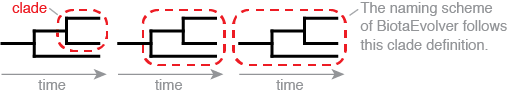
\includegraphics{images/clade_definitions.png}
\caption{}
\end{figure}

In BiotaEvolver, clades are defined by the root node for the purpose of
assigning species identifiers. The species at the root node is: * the
least recent common ancestor of all species in the tree, and * typically
introduced to a BiotaEvolver model using the \texttt{introduce\_species}
function.

The clades of the first 26 species are labeled alphabetically from A to
Z. The next 26 are labeled AB thru AZ.

1-26: A to Z 27-53: AA to AZ BA to BZ ... AAA to AAZ ABA to ABZ ACA to
ACZ

\subsubsection{Species number}\label{species-number}

Species are numbered sequently by clade beginning with 0.

In the example tree below, species A0 produced 4 child species. Only one
species, B0 exists in clade B because child species were not produced by
B0.

\begin{figure}
\centering
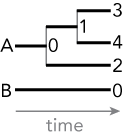
\includegraphics{images/species_number.png}
\caption{}
\end{figure}

    \subsubsection{Click here for more Landlab
tutorials}\label{click-here-for-more-landlab-tutorials}


    % Add a bibliography block to the postdoc
    
    
    
    \end{document}
